\documentclass[aspectratio=169,11pt]{beamer}

\usetheme{Madrid}
\usecolortheme{default}
\setbeamertemplate{navigation symbols}{}
\setbeamertemplate{footline}[frame number]

\usepackage{amsmath,amssymb}
\usepackage{booktabs}
\usepackage{tikz}
\usetikzlibrary{arrows.meta,positioning,shapes.geometric}

\title[QAgent]{QAgent: A Question-Generating Agent for Mathematical Research}
\subtitle{From paper reading to QED-ready theorem-level problems}
\author{QAgent Project}
\date{\today}

\newcommand{\qedready}{QED-ready}
\newcommand{\DeepMode}{Deep Mode}
\newcommand{\BatchMode}{Batch Mode}

\begin{document}

\begin{frame}
  \titlepage
\end{frame}

\begin{frame}{Core Objective}
  \begin{block}{What is QAgent trying to do?}
    Given a small collection of mathematical papers, QAgent generates theorem-level research problems that can be handed to GPT-Pro or a QED-like proving agent.
  \end{block}

  \vspace{0.4em}
  QAgent is not designed to produce vague open-problem titles. Its final output should include:
  \begin{itemize}
    \item a precise model, object class, assumptions, and conclusion;
    \item a problem decomposable into lemmas, estimates, and compactness steps;
    \item survey and duplicate-risk evidence;
    \item proof guidance, verification rules, feasibility analysis, and metadata;
    \item a realistic path toward a small publishable mathematical result.
  \end{itemize}
\end{frame}

\begin{frame}{Why Not Just Ask an AI Directly?}
  Direct prompting from abstracts often produces low-quality questions:
  \begin{itemize}
    \item \textbf{Keyword splicing:} ``regularity'' becomes a generic regularity problem.
    \item \textbf{Theorem reproduction:} the main theorem of the input paper is repackaged as a new problem.
    \item \textbf{Template titles:} for example, ``Sharp threshold for the main regularity mechanism''.
    \item \textbf{Wrong-domain mechanisms:} no-neck, varifolds, Yamabe, or De Giorgi appear where they do not belong.
    \item \textbf{No proof route:} the problem sounds interesting but has no first lemma or plausible proof sprint.
  \end{itemize}

  \vspace{0.4em}
  QAgent is built around quality gates rather than one-shot generation.
\end{frame}

\begin{frame}{System Architecture}
  \centering
  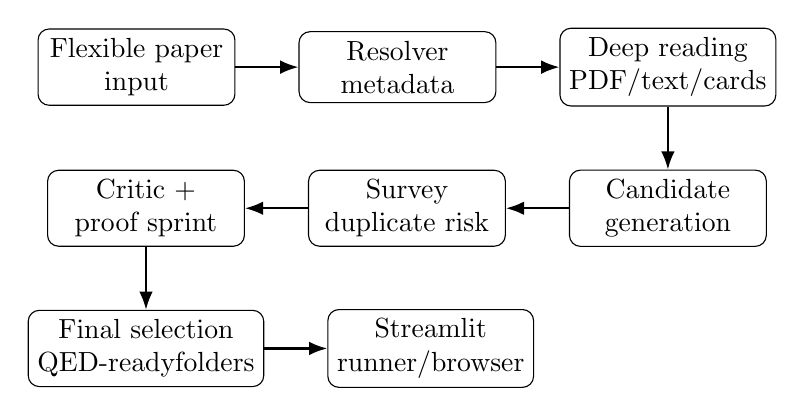
\begin{tikzpicture}[
    node distance=0.8cm,
    box/.style={draw, rounded corners, align=center, minimum width=2.5cm, minimum height=0.75cm},
    arrow/.style={-Latex, thick}
  ]
    \node[box] (input) {Flexible paper\\input};
    \node[box, right=of input] (resolve) {Resolver\\metadata};
    \node[box, right=of resolve] (read) {Deep reading\\PDF/text/cards};
    \node[box, below=of read] (cand) {Candidate\\generation};
    \node[box, left=of cand] (survey) {Survey\\duplicate risk};
    \node[box, left=of survey] (critic) {Critic +\\proof sprint};
    \node[box, below=of critic] (final) {Final selection\\\qedready folders};
    \node[box, right=of final] (ui) {Streamlit\\runner/browser};

    \draw[arrow] (input) -- (resolve);
    \draw[arrow] (resolve) -- (read);
    \draw[arrow] (read) -- (cand);
    \draw[arrow] (cand) -- (survey);
    \draw[arrow] (survey) -- (critic);
    \draw[arrow] (critic) -- (final);
    \draw[arrow] (final) -- (ui);
  \end{tikzpicture}
\end{frame}

\begin{frame}{Two Operating Modes}
  \begin{columns}[T]
    \begin{column}{0.48\textwidth}
      \begin{block}{\DeepMode}
        \begin{itemize}
          \item For 1--10 papers.
          \item Quality is prioritized over speed.
          \item Attempts metadata, PDF, and full-text reading.
          \item Extracts theorem, proof, method, limitation, and gap cards.
          \item Runs survey, critic review, and proof sprints.
          \item Intended for final theorem-level problem generation.
        \end{itemize}
      \end{block}
    \end{column}
    \begin{column}{0.48\textwidth}
      \begin{block}{\BatchMode}
        \begin{itemize}
          \item For 11--60 papers.
          \item Fast screening only.
          \item Outputs are marked lower confidence.
          \item Recommends which papers deserve Deep Mode.
          \item Not advertised as final SCI-level QED-ready generation.
        \end{itemize}
      \end{block}
    \end{column}
  \end{columns}
\end{frame}

\begin{frame}{Deep Reading Stage}
  Before asking for research questions, QAgent tries to understand the paper mechanism:
  \begin{itemize}
    \item \texttt{paper\_profile.json}: title, authors, model class, objects, methods, confidence.
    \item \texttt{theorem\_cards.json}: theorem labels, assumptions, conclusions, dimension, boundary conditions.
    \item \texttt{proof\_cards.json}: proof strategy, key lemmas, key estimates, fragile steps.
    \item \texttt{method\_cards.json}: reusable tools such as blow-up, monotonicity, Caccioppoli, compactness.
    \item \texttt{limitation\_cards.json}: dimension restrictions, smoothness, smallness, missing rates.
    \item \texttt{gap\_cards.json}: possible research gaps derived from theorem and limitation cards.
  \end{itemize}

  \vspace{0.4em}
  If only metadata or abstract is available, final outputs must be lower confidence.
\end{frame}

\begin{frame}{Candidate Generation: From Templates to Mechanisms}
  The old risk was overfitting to transfer templates.

  \vspace{0.5em}
  QAgent now uses a two-level transfer structure:
  \begin{enumerate}
    \item \textbf{Parent patterns:} perturbation, setting, dynamic, compactness/defect, quantitative, sharpness, low-regularity, proof-module.
    \item \textbf{Detailed TP patterns:} subpatterns and examples, not mandatory templates.
  \end{enumerate}

  \vspace{0.5em}
  Each strong candidate should explain:
  \begin{itemize}
    \item the source theorem or proof method;
    \item the target model;
    \item one primary new obstruction;
    \item why the old proof may survive;
    \item the smallest publishable theorem.
  \end{itemize}
\end{frame}

\begin{frame}{Domain Gate}
  Specialized proof mechanisms are allowed only in the right mathematical domain.

  \begin{block}{Examples}
    \begin{itemize}
      \item No-neck, bubble tree, and energy identity only for concentration or bubbling problems.
      \item Varifold compactness, tangent cones, and sheeting only for GMT, phase-field limits, currents, or minimal surfaces.
      \item De Giorgi iteration only for PDE regularity problems where level-set iteration is relevant.
      \item Yamabe, Green functions, and positive mass only for conformal or Riemannian geometry.
      \item Dispersive estimates only for wave, Schrodinger, or related dispersive PDE.
    \end{itemize}
  \end{block}

  Metadata now includes:
  \[
    \texttt{domain\_gate},\quad
    \texttt{forbidden\_mechanisms\_avoided},\quad
    \texttt{wrong\_domain\_mechanism\_penalty}.
  \]
\end{frame}

\begin{frame}{Theorem-Level Gate}
  The final \texttt{problem\_statement.tex} must be a clean theorem-level problem:

  \begin{itemize}
    \item a specific title;
    \item a concrete model: PDE, energy, variational problem, geometric object, or flow;
    \item a concrete setting: ball, bounded domain, manifold, half-ball, varifold setting, etc.;
    \item a concrete object class: weak solution, minimizer, stable critical point, integral current, etc.;
    \item explicit assumptions: dimension, regularity, boundary conditions, energy bounds, stability, smallness;
    \item a concrete conclusion: estimate, compactness, regularity, uniqueness, counterexample, or sharpness.
  \end{itemize}

  \vspace{0.4em}
  The \texttt{q} environment must not contain meta text such as ``Generated from metadata'', ``QED suitability'', or ``choose assumptions to match the paper''.
\end{frame}

\begin{frame}{Survey and Duplicate-Risk Gate}
  In Deep Mode, every candidate must receive a candidate-level survey report:

  \begin{itemize}
    \item at least eight search queries;
    \item exact title query, model + theorem type, model + conclusion, author + related theorem;
    \item public metadata sources: local metadata, Crossref, OpenAlex, arXiv, Semantic Scholar;
    \item no Google Scholar scraping;
    \item classification: reproduction, proof module, likely known, transfer, new theorem-level, or too vague.
  \end{itemize}

  \vspace{0.4em}
  High duplicate-risk candidates cannot be final selected.
\end{frame}

\begin{frame}{Critic Review and Proof Sprint}
  Each refinement round runs a proof sprint for every remaining candidate:

  \begin{enumerate}
    \item theorem-level restatement;
    \item key estimate or compactness lemma;
    \item 5--10 step proof attempt;
    \item where the input paper method is used;
    \item where the method may fail in the new setting;
    \item whether failure suggests a counterexample or sharpness version;
    \item QED/GPT-Pro attackability score;
    \item SCI publishable potential score;
    \item keep/remove reason.
  \end{enumerate}

  \vspace{0.4em}
  If the proof route is simply ``apply a known theorem directly'', the candidate is removed.
\end{frame}

\begin{frame}{Final Output Structure}
  Each final selected question becomes a \qedready folder:

  \begin{itemize}
    \item \texttt{problem\_statement.tex}
    \item \texttt{additional\_prove\_human\_help\_global.md}
    \item \texttt{additional\_verify\_rule\_global.md}
    \item \texttt{survey\_queries.md}
    \item \texttt{feasibility\_analysis.md}
    \item \texttt{metadata.json}
  \end{itemize}

  \vspace{0.4em}
  The main UI shows only the final selected problems, not candidate surveys or refinement logs.
\end{frame}

\begin{frame}{Runner UI}
  \begin{itemize}
    \item Paste flexible paper entries.
    \item Choose Deep Mode or Batch Mode.
    \item Set the number of papers \(n\), refinement rounds \(a\), and final questions \(b\).
    \item Click \textbf{Run Agent}.
    \item The backend uses Codex CLI.
    \item The UI shows blue ``running'', green ``completed'', or red ``failed'' status.
    \item The output browser shows papers by title and questions by selected-question title.
  \end{itemize}

  \vspace{0.4em}
  The current system does not call the OpenAI API and does not automate the GPT-Pro web UI.
\end{frame}

\begin{frame}{Recent Quality Improvement}
  We found that the active transfer catalog was too specialized. In particular, energy identity and no-neck language could contaminate unrelated papers.

  \vspace{0.5em}
  Changes made:
  \begin{itemize}
    \item changed the transfer catalog from a hard template to an idea source;
    \item added eight parent transfer patterns;
    \item replaced ``Energy Identity / No-Neck'' with ``Concentration / Defect-Control'';
    \item added a domain gate;
    \item reduced the weight of transfer-pattern fit;
    \item added wrong-domain mechanism penalty;
    \item connected the changes through runner prompt, validator, and hard review.
  \end{itemize}
\end{frame}

\begin{frame}{How We Verified the Change}
  We checked whether the changes actually affect the runtime pipeline:

  \begin{enumerate}
    \item \textbf{Catalog:} old TP19 title is gone; domain-gate rules are present.
    \item \textbf{Question prompt:} candidates must include \texttt{domain\_gate}.
    \item \textbf{Runner prompt:} Codex no longer sees ``must match one primary pattern''.
    \item \textbf{Validator:} new pattern fields enter the candidate quality audit.
    \item \textbf{Hard review:} pattern fit gives only a small bonus, not a hard gate.
    \item \textbf{Tests:} candidate validator, hard review, and runner prompt tests pass.
  \end{enumerate}
\end{frame}

\begin{frame}{Current Limitations}
  \begin{itemize}
    \item Output quality still depends heavily on full-text access and theorem-card extraction.
    \item Online survey uses public metadata sources and cannot replace a true literature review.
    \item GPT-Pro web interaction is a handoff, not automatic browser control.
    \item Batch Mode is screening only.
    \item Final theorem statements still need validator checks and human spot checks.
  \end{itemize}
\end{frame}

\begin{frame}{Next Steps}
  \begin{enumerate}
    \item Improve PDF, arXiv, and CVGMT full-text fetching.
    \item Make theorem-card extraction more reliable.
    \item Improve source-by-source logging for online survey.
    \item Add more user feedback examples of bad generated questions.
    \item Run Deep Mode on 1--3 papers as a high-quality demo.
    \item Compare QAgent scores against human proof-sprint judgments.
  \end{enumerate}
\end{frame}

\begin{frame}{Takeaway}
  \begin{block}{Main idea}
    QAgent first reads the paper mechanism, then generates candidates, surveys them, criticizes them, runs proof sprints, and only then selects final theorem-level problems.
  \end{block}

  \vspace{0.5em}
  The intended final problems should be:
  \begin{itemize}
    \item theorem-level and self-contained;
    \item not direct restatements;
    \item not template-driven;
    \item supported by a concrete new obstruction;
    \item plausible for QED/GPT-Pro assisted proof development;
    \item potentially publishable as small SCI-level results.
  \end{itemize}
\end{frame}

\end{document}
